\documentclass[a4paper, 14pt]{article} 
\usepackage[utf8]{inputenc}
\usepackage[T2A]{fontenc} 
\usepackage[english, russian]{babel}  
\usepackage[top = 20 mm, 
            bottom = 20 mm, 
            left = 30 mm, 
            right = 30 mm]{geometry}
\usepackage{indentfirst}
\usepackage{graphicx} 
\setlength{\parindent}{12.5 mm}
\usepackage{setspace}
\setstretch{1}
\pagestyle{headings}
\usepackage{fancyhdr}
\begin{document}

\begin{center}
{\raggedright УДК 519.715\\ \\ \centering\bf ПОСТРОЕНИЕ ГРАФА ПЕРЕХОДОВ\\ 
ПОСЛЕДОВАТЕЛЬНОСТНОЙ СХЕМЫ\\
С ПРИМЕНЕНИЕМ SAT-РЕШАТЕЛЯ}
\\
Иванов Иван Иванович
\\
кандидат технических наук, доцент
\\
доцент, Томский государственный университет
\\
Россия, Томск
\\
Петров Петр Петрович
\\
студент, Томский государственный университет
\\
Россия, Томск
\end{center}

Аннотация. Рассматривается подход к построению графа
переходов последовательностной схемы. Исследуется метод,
основанный на использовании SAT-решателя. Для построения графа
переходов определяются возможные переходы между состояниями
последовательной схемы и используются предварительные
вычисления, основанные на троичном и двоичном моделировании,
значительно сокращающие объем вычислений. Также
рассматривается построение на основе графа переходов
последовательностей, обеспечивающих заданные переходы схемы.
Компьютерные эксперименты показали эффективность
предложенного метода построения графа переходов с применением
SAT-решателя.

Ключевые слова: граф переходов, троичное моделирование,
SAT-решатель, последовательностная схема, переходная
последовательность.
\newline

В работе рассматривается подход к построению графа переходов
синхронной последовательностной схемы. Построение графа,
основанное на использовании SAT-решателя, исследуется подробно.
Представлены результаты компьютерных экспериментов для
предложенного метода построения графа переходов, применяющего
SAT-решатель. Также кратко рассматривается решение задачи
построения последовательности входных векторов, обеспечивающей
переход схемы в одно из состояний заданного множества, по графу
переходов. 


Рассмотрим синхронную последовательностную схему с $n$
входами, $m$ выходами и $p$ элементами памяти (триггерами).
$X = {x_1, ..., x_n}$ - входные переменные схемы, $Y = {y_1, ..., y_m}$ - ее
выходные переменные, $Z = {z_1, ..., z_p}$ – внутренние переменные
схемы.

Назовем \textit{графом переходов последовательностной схемы} ориентированный граф, у которого вершины сопоставлены состояниям схемы и есть дуга из вершины $i$ в вершину $j$ тогда и только тогда, когда в схеме существует одношаговый переход из состояния, соот-ветствующего вершине $i$, в состояние, соответствующее вершине $j$, при каких-либо значениях входных переменных.

На рисунке 1 представлена комбинационная составляющая С
последовательностной схемы. При построении графа переходов
рассматривается только та часть схемы, которая необходима для
получения функций переходов, выходы схемы не рассматриваются.
Поэтому структурное описание комбинационной составляющей,
используемой для получения графа переходов, упрощается (рисунок
2).
\begin{figure}[h]
\begin{minipage}[h]{0.49\linewidth}
\center{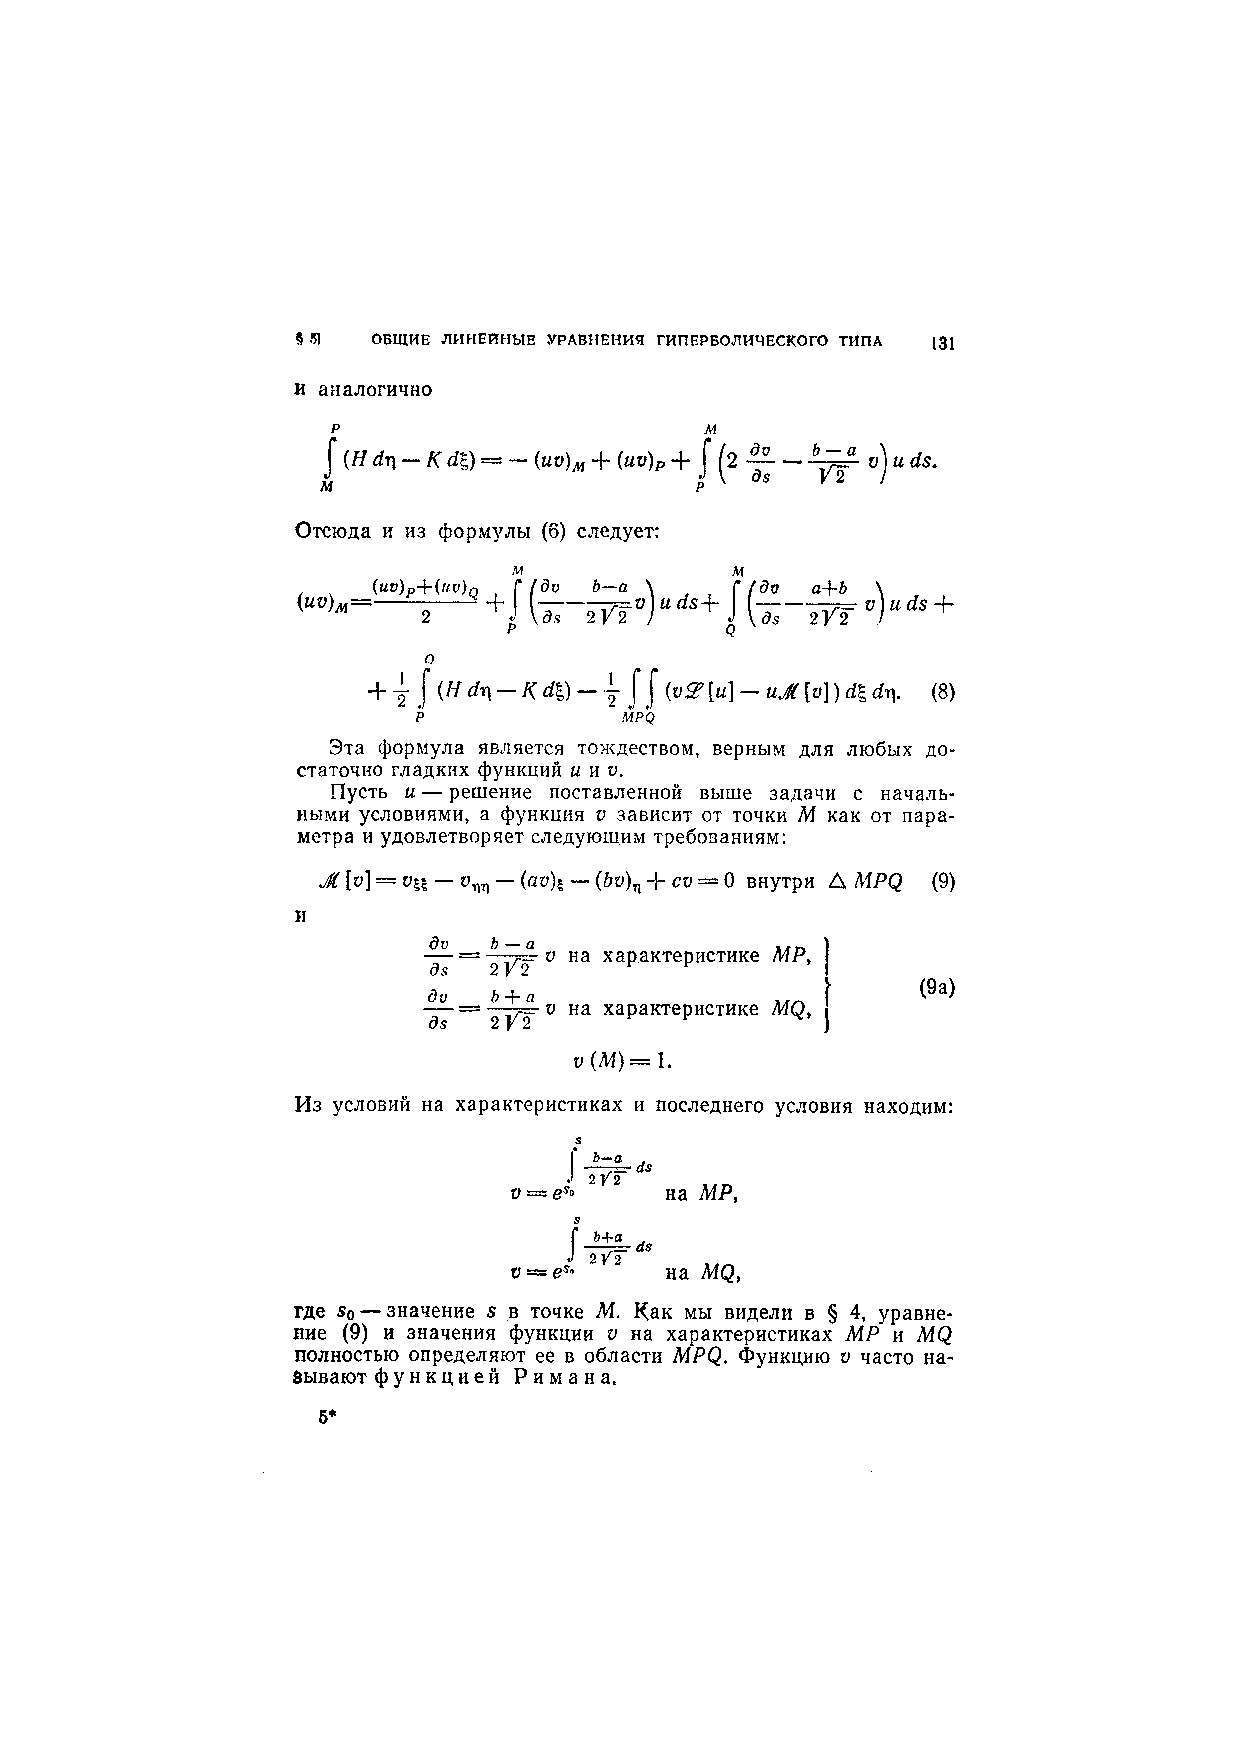
\includegraphics[width=0.5\linewidth]{1.jpg} \\ Рисунок 1 – Ирис setosa}
\end{minipage}
\hfill
\begin{minipage}[h]{0.49\linewidth}
\center{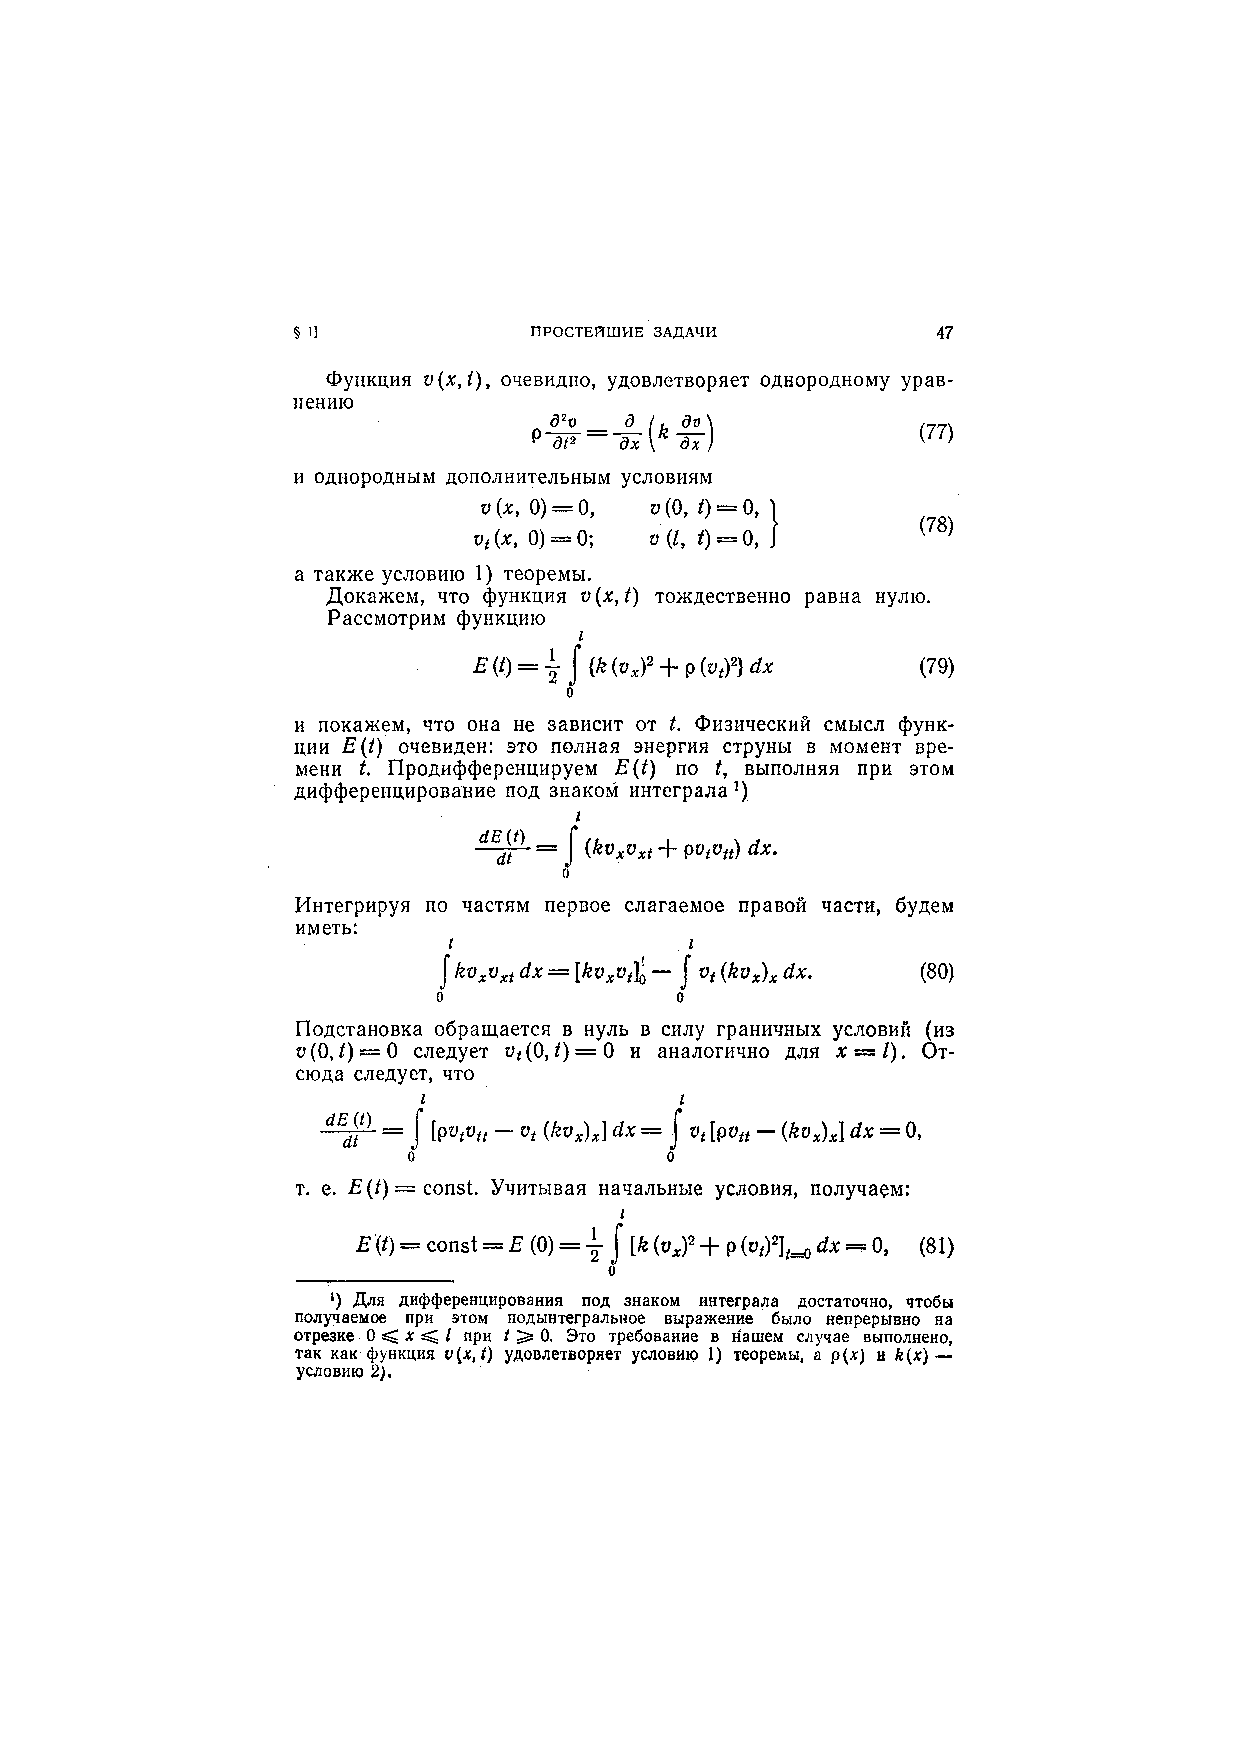
\includegraphics[width=0.5\linewidth]{2.jpg} \\ Рисунок 2 - Ирис virginica}
\end{minipage}
\label{ris:image1}
\end{figure}

В схеме с рисунка 2 можно исключить все элементы, не свя-занные с ее выходами, то есть с входами триггеров последователь-ностной схемы.

Система функций переходов последовательностной схемы имеет вид:
\begin{equation}
    z^t_{j}=\psi_{j}(x^t_{1},...,x^t_{n},z^{t-1}_{1},...,z^{t-1}_{p}),j=\overline{1,p}.
\end{equation}

Будем представлять полное состояние схемы вектором ($\alpha,\delta$), где $\alpha$ - вектор значений входных переменных X, а $\delta$ - вектор значе-ний внутренних переменных Z.
Двоичный вектор $\tau^i = (\tau^i_{1},\dots,\tau^i_{p}$
значений переменных Z будем
называть кодом состояния $q_{i}$. Q = $\{q_{1},\dots,q_{t}\}$, где t = $2^p$, – множество всех состояний схемы

Рассмотрим общий подход к построению графа переходов по-следовательностной схемы предложенный в работах [1, 2] и других.

Представленные свойства определены в [3].
Рассмотрим подробнее следующее свойство, сформулированное
в [3], используемое на 2-ом шаге сокращения вычислений.

\textit{Пусть выполнено точное троичное моделирование функций переходов системы (1) на векторе ($\alpha,\delta$), представляющем полное состояние, и получен вектор значений внутренних переменных $\delta'$. $\delta'$ представляет минимальный покрывающий интервал множества булевых векторов значений переменных Z, а не точное множество этих векторов. Таким образом, множество состояний схемы до-стижимых за один шаг из множества N($\alpha,\delta$) может быть под-множеством множества N($\delta'$). 
}\\


\textbf{Результаты экспериментов}

Для проверки эффективности предложенного метода построе-ния графа переходов последовательностной схемы, использующего SAT-решатель, были проведены эксперименты на бенчмарках. Экс-перименты проводились на контрольных примерах (бенчмарках) ISCAS’89, представляющих последовательностные схемы. Для оце-нивания работы исследуемого метода при проведении эксперимен-тов для различных бенчмарок измерялось время построения графа переходов, а также процент определяемых значений элементов мат-рицы M на каждом шаге предварительных вычислений. Результаты компьютерных экспериментов представлены в таблице 1. 

\begin{center}
    Таблица 1 – Результаты ранжирования рисков экспертной группой
\end{center}
\begin{table}[h]
\centering
\begin{tabular}{|p{1cm}|p{0.8cm}|p{0.8cm}|p{1.1cm}|p{1.1cm}|p{1.5cm}|p{1.7cm}|p{1.7cm}|p{1.6cm}|}
\hline\centering
\fontsize{7}{10}\selectfontБенч-марки & \centering\fontsize{7}{10}\centering\selectfontВходы\newline(\#) & \centering\fontsize{7}{10}\selectfontВыходы\newline(\#) & \centering\fontsize{7}{10}\selectfontЭлементы памяти\newline(\#) & \centering\fontsize{7}{10}\selectfontЭлементы\newline(\#) & \centering\fontsize{7}{10}\selectfontСреднее время построения графа (сек.) & \centering\fontsize{7}{10}\selectfontОпределенные переходы на шаге 1\newline(только 1)\newline(\%) & \centering\fontsize{7}{10}\selectfontОпределенные переходы на шаге 2\newline(только 0)\newline(\%) & \fontsize{7}{10}\selectfontСоотношение 0 и 1 в матрице М \newline (\#0,\#1)\\
\hline
S27 & 4 & 1 & 3 & 10 & 0,01 & 17,19 & 31,25 & 31;33 \\
\hline
S386 & 7 & 7 & 6 & 159 & 1,01 & 2,15 & 92,77 & 3800;296 \\
\hline
S832 & 18 & 19 & 5 & 287 & 7,60 & 11,13 & 61,23 & 710;314 \\
\hline
S510 & 19 & 7 & 6 & 211 & 21,84 & 2,46 & 97,36 & 3995;501\\
\hline
S1488 & 8 & 19 & 6 & 653 & 4,82 & 3,13 & 82,25 & 3369;727\\
\hline
\end{tabular}
\end{table}

В таблице представлены следующие данные: имя бенчмарки, количество входов, выходов, элементов памяти и элементов схемы; среднее время построения графа переходов схемы (по трем экспе-риментам); процент существующих одношаговых переходов в гра-фе, определенных на шаге 1 предварительных вычислений, процент не существующих одношаговых переходов, определенных на шаге 2 предварительных вычислений, и соотношение 0 и 1 в полученной матрице M. 

Шаги предварительных вычислений в экспериментах для рас-смотренных бенчмарок определили от 48,44\% до 99,82\% одношаго-вых переходов (существующих и не существующих в графе). Шаг 2 предварительных вычислений, выполненный с помощью троичного моделирования, позволил определить большую часть одношаговых переходов, отсутствующих в графе. Значительная часть всех одно-шаговых переходов графа вычислена с помощью шагов 1 и 2 пред-варительных вычислений. Графы переходов для схем среднего раз-мера построены за несколько секунд.  
\begin{center}
{\bf Список литературы}
\end{center}
\newline
1. Иванов И.И. Построение графа переходов последовательностной схемы // Современные проблемы физико-математических наук: материалы IV Всероссийской науч.-практ. конф. с международным участием, (22 – 25 ноября 2018 г., г. Орёл). - Орел: ОГУ им. И.С. Тургенева, 2018. – Ч. 1. – С. 230 – 235.
\newline
2. Ivanov I. Three-Value Simulation of Combinational and Sequential Circuits and its Applications // 2020 IEEE Moscow Workshop on Electronic and Networking Technologies (MWENT). Moscow, Russia. 11-13 March 2020. - 7 pp.
\newline
3. Иванов И.И. Интервальные расширения булевых функций и троичное моделирование последовательностных схем // Таврический научный обозреватель. - 2017. - №5 (22). - С. 208-220.
\newline
4. Иванов И.И. Троичное моделирование комбинационных и синхронных последовательностных схем // Современные проблемы физико-математических наук / материалы V Всероссийской науч.-практ. конф. с международным участием, (26 – 29 сентября 2019 г., г. Орёл). – Орел: ОГУ им. И.С. Тургенева, 2019. – С. 274 – 281.
\end{document}